\documentclass[12pt, a4paper]{article}
\setlength{\parindent}{0pt}
\usepackage[utf8]{inputenc}
\usepackage[spanish]{babel}
\usepackage{hyperref}
\usepackage{graphicx}
\usepackage{wrapfig}
\usepackage{caption}
\usepackage{subcaption}
\usepackage{multirow} 
\usepackage{ textcomp }
\usepackage[bottom]{footmisc}
\usepackage{ amssymb }
\usepackage{amsmath}

\begin{document} 
\title{Trabajo Práctico Final\\ Machine Learning} 
\author{Bianchi, Gabina Luz} 
\maketitle

\section*{Ejercico A}
La implementación utilizada del método \textit{support vector machine} es \textit{SVM Light} \footnote{Se puede descargar de aquí: \url{http://svmlight.joachims.org/}}. \\
Primero se procedió a particionar el conjunto de datos \textit{heladas} (el único conjunto de datos que se utiliza en este trabajo) en 10, manteniendo la proporción de puntos de cada clase\footnote{En realidad, no fue posible mantener exacta la proporción de puntos de cada clase, dado que existen en el conjunto de datos original, 184 punto de clase 1 y 316 pertenecientes a la clase 0. Se optó por hacer algunos conjuntos con 19 puntos de clase 1 y 31 de clase 0, y otors con 18 puntos de clase 1 y 32 de clase 0.}, y armar los datos necesarios para poder aplicar validación cruzada. Luego se aplicaron los algoritmos pedidos, ajustando los parámetros correspondientes. 
\subsection*{C4.5 y Naive Bayes}

\begin{figure}
    \centering
	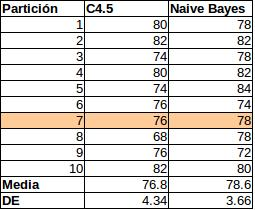
\includegraphics[scale=0.8]{tabla1}
	\caption{Porcentaje de aciertos en cada una de las particiones utilizando C4.5 y Naive Bayes con normales.}
\end{figure}


Los primeros algoritmos aplicados fueron C4.5 y Naive Bayes con normales, dado que no necesitaban ajustar parámetros.  Los resultados se encuentran en la tabla de la Figura 1. En naranja se marca la partición que obtuvo resultados más similares a las medias. El valor que se considera para definir cuál algoritmo presenta, aprentemente, un resultado mejor, es la media. Por lo tanto, en este caso, se concluye que Naive Bayes predice mejor que C4.5.


\subsection*{Support Vector Machine}

\subsubsection*{Kernel lineal}

Con la información obtenida a partir de los resultados anteriores se procedió a ajustar el parámetro \textit{C} para SVM con kernel lineal, de modo de superar los niveles de aciertos. Se utilizó la partición 7, por ser ésta la que obtuvo resultados más parecidos a las medias obtenidas para los algoritmos mencionados anteriormente.\\
Para comenzar la búsqueda del valor del parámetro \textit{C}, primero se realizaron las pruebas que se muestran en la tabla de la Figura 2.

 \begin{figure}
    \centering
	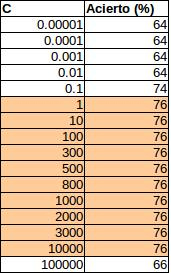
\includegraphics[scale=0.8]{tabla2}
	\caption{Porcentaje de aciertos en la partición 7 con SVM lineal, variando el valor de \textit{C}.}
\end{figure}

Allí se hace un barrido para posibles valores de \textit{C}, y se observa que utilizando valores que se encuentran entre 1 y 10000 se obtiene el mismo resultado (para una partición particular). Por lo tanto, para seguir con la búsqueda se optó por elegir algunos posibles valores de \textit{C} en el rango mencionado (evitando los valores muy altos), y aplicar el algoritmo a cada una de las particiones generadas, calculando la media y la desviación estándar. Los resultados se presentan en la tabla de la Figura 3. Allí se encontró que el mejor resultado se da para \textit{C} = 30, con una media de 80.4 \% de aciertos y una desviación estándar de 4.5. Se podría haber optado por elegir el resultado logrado con \textit{C} = 15, ya que si bien presenta una media menor, la desviación estándar también lo es. 

 \begin{figure}
    \centering
	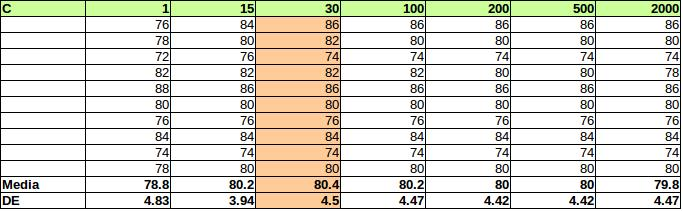
\includegraphics[scale=0.8]{tabla3}
	\caption{Porcentaje de aciertos en cada partición con SVM lineal, variando el valor de \textit{C}.}
\end{figure}



\subsubsection*{Kernel polinomeal}
El kernel no lineal elegido es el polinomeal. Para utilizarlo, además de ajustar el parámetro \textit{C}, se debe ajustar el grado \textit{D} del polinomeo utilizado. Siendo que 2 es el valor más popular para el grado, primero se hizo un barrido para los posibles valores de \textit{C} (análogo al hecho anteriormente), fijando \textit{D} = 2. En la tabla de la Figura 4 se presentan los resultados obtenidos para la partición 7.

 \begin{figure}
    \centering
	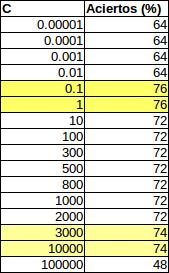
\includegraphics[scale=0.8]{tabla4}
	\caption{Porcentaje de aciertos en la partición 7 con SVM polinomeal con grado 2.}
\end{figure}

Allí se observa que los mejores resultados se obtienen para \textit{C} = 0.1, \textit{C} = 1, \textit{C} = 3000 y \textit{C} = 10000. Luego se procedió a fijar esos valores de \textit{C} y variar el parámetro \textit{D} en un rango de 2 a 300. Los resultados se presentan en la tabla de la Figura 5.

 \begin{figure}
    \centering
	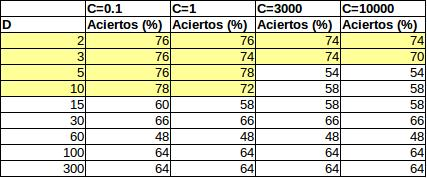
\includegraphics[scale=0.9]{tabla5}
	\caption{Porcentaje de aciertos en la partición 7 con SVM polinomeal.}
\end{figure}

En dicha tabla se puede observar que los mejores resultados se obtienen para grados pequeños, entre 2 y 10. Posiblemente para polinomeos con grados muy altos se haga sobreajuste. \\
Finalmente, con los \textit{C} en los cuales se obtuvo mejor resultado (0.1 y 1), se corrió el algoritmo para cada partición variando el \textit{D} entre 2,3,4 y 5. En la tabla de la Figura 6 se presentan los resultados obtenidos. El mejor caso es el logrado con \textit{C} = 1 y \textit{D} = 5, con un 81\% de aciertos y una desviación estándar de 3.56.

 \begin{figure}
    \centering
	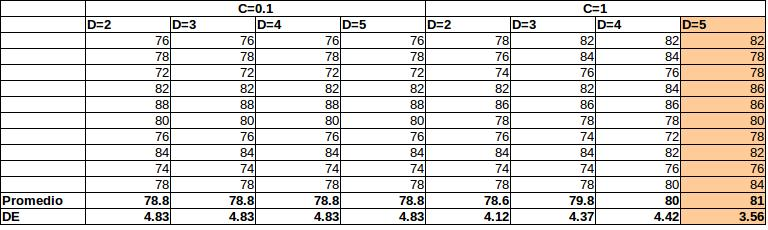
\includegraphics[scale=0.8]{tabla6}
	\caption{Porcentaje de aciertos obtenidos con SVM polinomeal para todas las particiones.}
\end{figure}

\subsection*{Resultados Finales}
En la tabla de la Figura 7 se presentan las medias y desviaciones estándares de los mejores resultados de los 4 algoritmos utilizados.


 \begin{figure}
    \centering
	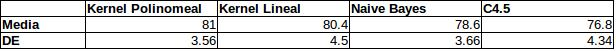
\includegraphics[scale=0.95]{tabla9}
	\caption{Media y desviación estándar del porcentaje de aciertos logrados con cada algoritmo utilizado.}
\end{figure}

\section*{Ejercicio B}

En este ejercicio se pide realizar dos \textit{t-test} con 95\% de confidencia entre algunos de los resultados obtenidos en la parte A.\\
En la tablas de la Figura 8 y la Figura 9 se encuentran los valores que se utilizaron para dichos tests. Los dos mejores resultados se obtuvieron utilizando SVM, con kernel polinomeal y con kernel lineal, respectivamente, mientras que el peor fue el logrado con C4.5.

 \begin{figure}
    \centering
	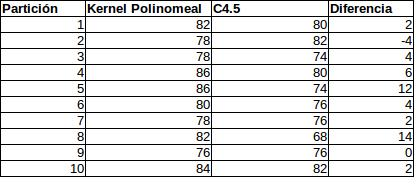
\includegraphics[scale=0.8]{tabla7}
	\caption{Valores utilizados para el \textit{t-test} entre el mejor y el peor resultado.}
\end{figure}
 \begin{figure}
    \centering
	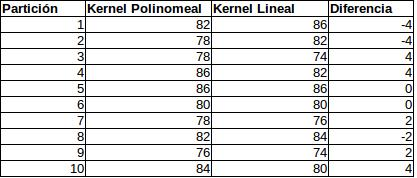
\includegraphics[scale=0.8]{tabla8}
	\caption{Valores utilizados para el \textit{t-test} entre el mejor y el segundo mejor resultado.}
\end{figure}


\bigskip

A continuación se presentan algunas consideraciones respecto a los tests realizados. \\
El parámetro $\bar{\delta}$ representa la media de las diferencias de aciertos observadas entre ambos algoritmos  (ver Figura 8 y Figura 9). Dado que el conjunto total de datos se particionó en 10, se tiene \textit{k} = 10,  siendo $\bar{\delta_i}$ la diferencia entre los aciertos para la partición \textit{i}, variando \textit{i}=1,...,\textit{k}. El parámatro $S_{\bar{\delta}}$, el cual representa una estimación de la desviación estándar, está definido como  $\sqrt{\frac {\sum_{i=1}^k (\bar{\delta_i} - \bar{\delta})^2}{k \ (k-1)}} $. Siendo que el test realizado es de 95\% de confidencia con 9 grados de libertad, se tiene $t_{N,k-1}  = 2.26 $.

\bigskip

Al comparar SVM con kernel polinomeal y C4.5 se tienen los siguientes resultados. \\

\[  \bar{\delta}  = 4.2 \]
\[    S_{\bar{\delta}} \approx 1.69 \]
\[ \bar{\delta} \pm  S_{\bar{\delta}} \  t_{N,k-1}  \approx 4.2 \pm 1.69 \  2.26  \approx [0.36; \ 8.03 ] \]

Esto se interpreta de la siguiente manera: hay un 95\% de posibilidad de que la media real de las diferencias de desempeño entre los dos algoritmos estudiados en este caso pertenezca al rango [0.36,8.03]. Por lo tanto, considerando que todos los valores en dicho intervalo son mayores a 0, se puede decir que hay un 0.95 de probabilidad de que el algoritmo SVM con kernel polinomeal (y los parámatros discutidos en el ejercicio A) tenga, en promedio, mayor cantidad de aciertos que el C4.5.\\

\bigskip

Por el contrario, al comparar ambos desempeños de SVM, se obtiene el resultado que se presenta a continuación. 

\[  \bar{\delta}  = 0.6 \]
\[    S_{\bar{\delta}} \approx 0.99 \]
\[ \bar{\delta} \pm S_{\bar{\delta}} \  t_{N,k-1}  \approx 0.6 \pm 0.99 \  2.26  \approx [-1.63; \ 2.83 ] \]

Esto significa que hay 0.95 de probabilidad de que la media real de la diferencia entre ambos algoritmos de SVM pertenezca al intervalo [-1.63, 2.83]. Por lo tanto, siendo que existen valores negativos, no se puede concluír que hay 0.95 de probabilidad de que el kernel polinomeal tenga, en promedio, mayor cantidad de aciertos que el kernel lineal.

\end{document}